\chapter{Introduction}

\section{Background}

Drug discovery is an expensive and long-term business. Summarized from 13 research articles published from 1980 to 2009, original estimates of the cost of drug development ranged more than 9-fold, from USD\$92 million cash (USD\$161 million capitalized) to USD\$883.6 million cash (USD\$1.8 billion capitalized) \citep{1431}. Discovering and developing a new molecular entity (NME) required 11.4 to 13.5 years using the R\&D performance productivity data from 13 large pharmaceutical companies across 2000 to 2007 \citep{716}. An recent report \citep{1427} reviewed the rates of NMEs introduction starting from 1827 through to the end of 2013, and found that two-thirds of NMEs are controlled by a handful of companies, and a growing number of NMEs are controlled by marketing organizations that have little or no internal drug discovery or development activities.

The process of modern drug discovery typically includes target identification, hit identification, lead optimization and clinical trials. A biological target is any system that can potentially be modulated by a molecule to produce a beneficial effect. A target could be a fundamental pathological pathway, altering which is expected to be curative or anti-symptomatic. Hits are compounds that have activity at a predetermined level against a target, but little else is known at this early stage. Leads are optimized hits that display strong potency and selectivity, physicochemical characteristics, and absorption, distribution, metabolism, excretion and toxicity (ADMET) properties. Successful candidate leads will then be submitted to the health authorities to get permission to conduct clinical investigations on animals and humans.

An essential ingredient of drug discovery is to discover inhibitory molecules for pharmaceutical protein targets of therapeutic interest. Take the HIV (Human Immunodeficiency Virus) virus for example \citep{296}. The virus comprises several protein enzymes, which play critical roles in viral replication. In HIV-infected cells, the viral reverse transcriptase reversely transcribes viral RNA into viral DNA, the viral integrase integrates viral DNA into human genomic DNA, and the viral protease assemblies viral RNA and viral proteins into a new virion. This replication cycle will be blocked if the viral proteins are inhibited. Such inhibitors are typically small compounds called ligands, which function through binding to the enzymatic or allosteric sites of target proteins.

Terminologically, screening refers to the process of discovering ligands that show activity towards certain proteins of interest. A library of compounds is routinely screened to shortlist candidate ligands. When this process is done \textit{in silico} using computer simulations, it is called virtual screening. Regarding the methods in use, virtual screening can be classified into structure-based virtual screening and ligand-based virtual screening. Their major difference lies in whether the target protein is present or absent. Structure-based virtual screening uses explicit knowledge of the target protein to suggest candidate protein-ligand complexes commonly via a method called docking, whereas ligand-based virtual screening does not encode target information but infers required characteristics of binders from known bioactive ligands.

To really aid drug discovery, a complete toolchain should include tools for both structure-based virtual screening (chapter 2) and ligand-based virtual screening (chapter 9), as well as relevant tools and studies, e.g. a web platform (chapter 3), visualization (chapter 4), drug design and synthesis (chapter 5), binding affinity prediction (chapters 6 and 7), pose generation error reduction (chapter 8), and others. Eventually these tools and studies become useful only when they are applied to real world problems, such as finding cures for influenza (chapter 10) and cancers (chapter 11).

\section{Motivation}

Drug discovery is economy driven \textit{per se}. Biochemical means are both cost- and time-inefficient. This highlights the need for cheaper and faster methods, and computer-aided drug discovery (CADD) thus comes into the scene. Complementing expensive laboratory experiments with cheap computer simulations is obviously the right way to go. Robust computational frameworks are indeed highly demanded by the industry in order to automate the early phases of modern drug discovery such as hit identification and lead optimization.

Although a large amount of CADD tools have been developed over recent decades, the majority of them, unfortunately, suffer from several notable problems. These tools 1) are commercial, selling at a price that most small enterprises and academic institutions cannot afford, 2) are proprietary and closed source, making third parties difficult to study the internal implementations or locate potential bugs, 3) conform to different standards and formats, resulting in weak data portability and information loss, 4) require intensive and tedious configurations and lack a friendly user interface, a great obstacle for new users to get started, 5) run rather slowly, incapable of utilizing the multi- and many-core architectures of modern computers, or even worse, 6) are declared dead immediately upon their initial release due to zero maintenance afterwards. In this thesis, we attempt to address these shortcomings.

\section{Objective}

We aim to develop a pragmatic and concise CADD toolchain, and ultimately apply it to the discovery of novel drugs. Keeping several key goals in mind, we design our toolchain to 1) be freely available to the general public, 2) be released under permissive open source licenses, 3) conform to official standards, 4) provide a responsive web version, 5) run reasonably fast, and 6) track bugs and issues and incorporate user feedback. We emphasize reproducibility, which has the potential to serve as a minimum standard for judging scientific claims when full independent replication of a study is not possible \citep{965}. Most importantly, we shall utilize our toolchain to discover potent drugs against certain diseases of therapeutic interest and hopefully save human lives.

\section{Contributions}

Figure \ref{thesis:contributions} highlights the overall contributions of this thesis.

\begin{figure}
\begin{center}
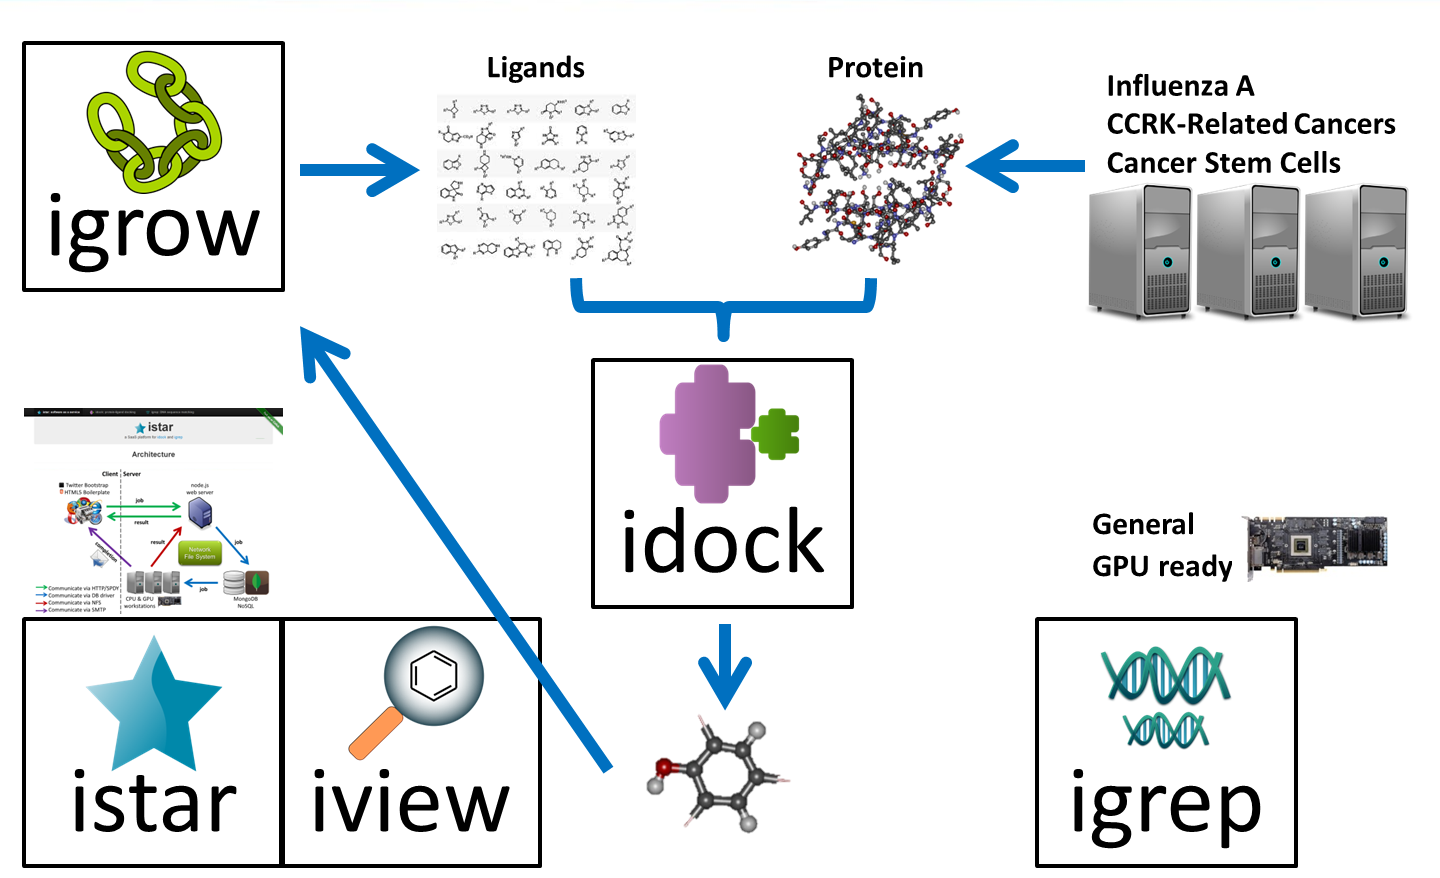
\includegraphics[width=\linewidth]{Contributions.png}
\end{center}
\caption{Contributions of this thesis.}
\label{thesis:contributions}
\end{figure}

In chapter 2, we have developed idock \citep{1153} as a multithreaded flexible ligand docking tool for native support of structure-based virtual screening in a superfast fashion. Based on the state-of-the-art AutoDock Vina, our idock substantially revises the numerical approximation model and enhances the fundamental implementation of various components with modern C++11 tricks. Notably, it encapsulates a novel feature for dimension reduction by detecting inactive torsions. Compared with AutoDock Vina \citep{595}, idock obtained a speedup of 3.3 in terms of CPU time and a speedup of 7.5 in terms of elapsed time on average, making it a very competitive tool. We have then used idock in a prospective virtual screening campaign of docking 10,938 drug-like ligands against HIV reverse transcriptase with minimal toxical side effects against four other human proteins for the treatment of AIDS. This project has been published \citep{1153}.

In chapter 3, we have developed istar \citep{1362} as a versatile SaaS (Software as a Service) web platform to promote software usage by a wide variety of users from different disciplines. Particularly, we have hosted idock on istar for large-scale prospective structure-based virtual screening. Our istar website supports three novel features: 1) filtering ligands by desired molecular properties and previewing the number of ligands to dock, 2) monitoring job progress in real time, and 3) visualizing docked conformations and outputting supplier information for easy purchasing. We have collected as many as 23,129,083 ligands, revamped our idock to version 2.0, and integrated RF-Score \citep{564} as an alternative rescoring function. We have shown that idock achieved comparable success rates while outperforming AutoDock Vina in terms of docking speed by at least 8.69 times and at most 37.51 times. In combination with RF-Score, istar managed to reproduce Pearson and Spearman correlation coefficients of as high as 0.855 and 0.859, respectively, between the experimental and the predicted binding affinity. We believe istar constitutes a step toward generalizing the use of docking tools beyond the traditional molecular modeling community. istar::idock is freely available at http://istar.cse.cuhk.edu.hk/idock. This project has been published \citep{1362}.%TODO: mention istar Google Analytics statistics.

In chapter 4, we have developed iview \citep{1366} as an easy-to-use interactive WebGL visualizer for protein-ligand complex to enable non-experts to quickly elucidate protein-ligand interactions in a 3D manner. As far as we are aware, iview is the only web visualizer that simultaneously utilizes GPU hardware acceleration and supports three pragmatic features: macromolecular surface construction, virtual reality effects, and PDBQT format parsing. Moreover, based on the feature-rich version of iview, we have also developed a concise version specifically for our idock web service on istar to aid online protein-ligand docking. This demonstrates the excellent portability of iview, which can be easily integrated into any bioinformatics application that requires interactive protein-ligand visualization. iview is freely available at http://istar.cse.cuhk.edu.hk/iview. This project has been published \citep{1366}.

In chapter 5, we have developed iSyn \citep{1409,1387} as an effective and efficient fragment-based drug design tool that generates desired \textit{de novo} compounds with promising potency and molecular mass to complement structure-based virtual screening. It features an evolutionary algorithm that creates novel ligands with drug-like properties and ensures synthetic feasibility with click chemistry. Interfacing with our fast molecular docking engine idock and our interactive WebGL visualizer iview, iSyn substantially reduces the drug candidate evaluation time and increases productivity. Benchmarking results of iSyn in generating novel inhibitors \textit{ex nihilo} of two important drug targets TbREL1 and CDK2 have proved its strength in significantly enhancing the predicted binding affinity of the best generated ligand by more than 3 orders of magnitude in potency within a reasonable time. iSyn is freely available at http://istar.cse.cuhk.edu.hk/iSyn.tgz. This project has been published \citep{1409,1387}.

%In chapter 6, we have presented a study

%In chapter 7, we have presented a study

%In chapter 8, we have presented a study

In chapter 9, we have proposed a pragmatic implementation of USR (Ultrafast Shape Recognition) \citep{1379} and its extension USRCAT (USR with Credo Atom Types) \citep{1331} based on our istar web platform in order to quickly and conveniently search for compounds structurally similar to a query ligand in terms of shape. Our molecular database is populated with more than 230 million diverse and representative conformers so as to reduce the possibility of missing compounds with similar shape to the query. We perform screening time analysis, based on which we exploit three levels of parallelism with a novel implementation of sum of absolute differences using AVX (Advanced Vector Extensions) to accelerate job execution. Our istar::USR supports multiple query ligands in SDF, MOL2, XYZ, PDB or PDBQT formats, and interfaces with our iview WebGL visualizer for interactive visualization of high-score hits. istar::USR is freely available at http://istar.cse.cuhk.edu.hk/usr. In addition, we have also briefly described USRT (USR with Torsions), the very first USR-like algorithm that can identify different conformations of the same ligand. One of its biggest applications is to circumvent the task of conformer generation.

It is worthwhile to highlight that all of the above CADD tools are free and open source under permissive licenses.

\section{Thesis Outline}

The thesis is organized into 12 chapters. Chapter 2 presents idock, our protein-ligand docking tool for fast structure-based virtual screening. Chapter 3 presents istar, our web platform for online CADD. Chapter 4 presents iview, our WebGL visualizer for convenient online visualization. Chapter 5 presents iSyn, our fragment-based drug design tool for \textit{in silico} synthesis of novel drug candidates. Chapter 6 presents RF::Cyscore. Chapter 7 presents RF-Score-v3, our accurate binding affinity prediction tool for crystal conformations. Chapter 8 presents RF-Score-v4, our accurate binding affinity prediction tool for docked conformations. Chapter 9 presents istar::USR, our implementation of ultrafast shape recognition methods on istar for ligand-based virtual screening. Chapter 10 presents our case study of influenza A H1N1. Chapter 11 presents our case study of CDK2-related cancers. Chapter 12 summarizes the thesis. The appendix lists my journal and conference publications in 2012 to 2014 in chronological order.

\chapterend
